\documentclass[12pt,a4]{article}

\usepackage{graphicx,amsmath,amssymb,amsthm, boxedminipage}

\usepackage{algorithm}
\usepackage{algpseudocode}


\newtheorem{theorem}{Theorem}%[section]
\newtheorem{proposition}[theorem]{Proposition}
\newtheorem{lemma}[theorem]{Lemma}
\newtheorem{corollary}[theorem]{Corollary}
\newtheorem{definition}[theorem]{Definition}

\newcommand{\scalar}[2]{\ensuremath{\langle #1, #2\rangle}}
\newcommand{\floor}[1]{\left\lfloor #1 \right\rfloor}
\newcommand{\ceil}[1]{\left\lceil #1 \right\rceil}
\newcommand{\norm}[1]{\|#1\|}
\newcommand{\pfrac}[2]{\left(\frac{#1}{#2}\right)}
\newcommand{\nth}[1]{#1\textsuperscript{th}}

% \newcommand{\nth}[1]{#1\textsuperscript{th}}
\newcommand{\E}{\mathop{\mathbb{E\/}}}
\newcommand{\N}{\mathbb{N}}

\newcommand{\R}{\mathbb{R}}

\newtheorem{exercise}[theorem]{Exercise}
\newtheorem{exerciseD}[theorem]{*Exercise}
\newtheorem{exerciseDD}[theorem]{**Exercise}

\let\oldexercise\exercise
\renewcommand{\exercise}{\oldexercise\normalfont}

\let\oldexerciseD\exerciseD
\renewcommand{\exerciseD}{\oldexerciseD\normalfont}

\let\oldexerciseDD\exerciseDD
\renewcommand{\exerciseDD}{\oldexerciseDD\normalfont}


 
\begin{document}

\author{NoCode}
\date{\today}

\title{CS 217 -- Algorithm Design and Analysis \\ 
  \vspace{3mm}
{\large	Shanghai Jiaotong University, Fall 2019\\
}
}
\maketitle

\noindent


\section{Bit Complexity, Recursion, and Dynamic Programming}

\subsection{Bit Complexity of Euclid's Algorithm}

We have proved that Euclid's algorithm for computing $\gcd(a,b)$ makes at most
$O(\log a)$ iterations. What is the overall running time? Each iteration computes
$u \mod v$ for some integers. This can be done by integer division. What is its running time?
There are very sophisticated algorithms, but python probably does not come with them. 
Recall the ``school method'' for dividing integers. Have a look at the pdf slides on the 
webpage for an illustration of the school method. It is especially simple if we are dealing
with binary numbers. If $a$ and $b$ have at most $n$ bits, then the school method 
has complexity $O(n^2)$.
\begin{exercise}
  Show the following, more precise bound of the school method for integer division:
  If $a$ has $n$ bits and $b$ has $k$ bits, then the school method can be implemented
  to run in $O( k(n-k))$ operations.
  
\paragraph{Solution} Since $b$ has $k$ bits, each time we implement a subtraction costs us $k$ operations. 
Also, for the school method, the divisor will move at least 1 bit right after a subtraction. 
During the whole process, the divisor will move at most $n-k$ times, since the divisor already has $k$ bits. 
Thus, it will costs at most $O(k(n-k))$ operations to implement school method for integer division. 
  
\end{exercise}

\begin{exercise}
  Show that the bit complexity of Euclid's algorithm, using the school method
  to compute $a \mod b$, is $O(n^2)$. That is,
  if $a$ and $b$ have at most $n$ bits, then $\gcd(a,b)$ makes $O(n^2)$ bit operations.\\
  
  In order to do so, here is python code of the Euclidean algorithm:
\begin{verbatim}
  def euclid(a,b):
    while (b > 0):
        r = a % b # so a = bu+r
        if (r == 0):
            return b
        s = b % r # so b = rv + s
        a = r
        b = s
    return a
\end{verbatim}
Don't be afraid to introduce notation! I recommend to let $n$ denote the number of bits of $a$.
Take some other letters for the number of bits in $b$ and so on.

\paragraph{Solution}

Let $n$ denote the number of bits of $a$. We already know that Euclid's algorithm 
for computing $\gcd(a,b)$ makes at most $O(n)$ iterations.
Now we first prove a lemma.
\paragraph{Lemma 1.1.2.1}
For $a_1, a_2, \ldots, a_m$ and $\sum_{i=1}^m a_i = n$, $\sum_{i=1}^{m} a_i(n-\sum_{j=1}^i a_j)$ has maximum value only when $a_1 = a_2 =\ldots = a_m$

\textbf{Proof.} To maximize
\begin{align*}
  \sum_{i=1}^{m} a_i(n-\sum_{j=1}^i a_j) &= n^2 - \sum_{i=1}^m(a_i\sum_{j=1}^i a_j)\\
  &= n^2 - \sum_{i=1}^m \sum_{j=1}^i a_i a_j 
\end{align*}
we need to minimize 
\begin{align*}
  \sum_{i=1}^m \sum_{j=1}^i a_i a_j &= \frac{a_1^2}{2} + \sum_{i=2}^m(\frac{2\sum_{j=1}^{i-1} a_j + a_i}{2}) + \sum_{i=1}^m \frac{a_i^2}{2} \\
  &= \frac{(n-1)^2}{2} + \frac{1}{2} \sum_{i=1}^m a_i^2
\end{align*}
Based on the mean value inequality, when $a_1 = a_2 =\ldots =a_m$, $\sum_{i=1}^m a_i^2$ has the minimum value, which means $\sum_{i=1}^{m} a_i(n-\sum_{j=1}^i a_j)$ has maximum value.

Now we come back to the problem. Suppose we need to do Euclid's algorithm for $m (1\leq m\leq n)$ iterations, and for every iterations we can shorten $a$ by $a_i$ bits. From the lemma, we can conclude that when $a_1 = a_2 = \ldots = a_m = \frac{n}{m}$ we would have the maximum operations which is the worst case.

Now consider the worst case, that is, we have to do the school method division for $m$ times, each time we can shorten the dividen by $t( = \frac{n}{m})$ bits.
Use the conclusion from \textbf{Exercise 1.}, we can write the total operations needed as below:
\begin{align*}
  \sum_{i=1}^m (n-it)t &= n^2 - t^2\sum_{i=1}^m i \\
  &= n^2 - \frac{n^2}{m^2} \frac{m(m+1)}{2}\\
  &= \frac{n^2}{2} - \frac{n^2}{2m}
\end{align*}

When $m = 1$, we have the worst case to compute gcd($a,b$), which is $O(n^2)$.
Thus, the bit complexity of Euclid's algorithm, using the school method
to compute $a \mod b$, is $O(n^2)$.

\end{exercise}

\subsection{Computing the Binomial Coefficient}

Next, we will investigate the binomial coefficient ${n \choose k}$, which 
you might also know by the notation $C^k_n$. The number ${n \choose k}$ is defined
as the number of subsets of $\{1,\dots,n\}$ which have size exactly $k$. 
This immediately shows that ${n \choose k}$ is $0$ if $k$ is negative or larger than $n$.
You might have seen the following recurrence:
\begin{align*}
 {n \choose k} & = {n-1 \choose k-1} + {n-1 \choose k} \textnormal{ if } n,k \geq 0 \ .
\end{align*}

\begin{exercise}[A Recursive Algorithm for the Binomial Coefficient]
  Using pseudocode, write a recursive algorithm computing
  ${n \choose k}$. Implement it in python! What is 
  the running time of your algorithm, in terms of $n$ and $k$? Would you say it is an efficient
  algorithm? Why or why not?
\end{exercise}
\paragraph{Solution}
\begin{verbatim}
 def Binomial(n, k):
    if (k > n or k < 0): 
        return 0
    elif (n == k or k == 0): 
        return 1
    else: 
        return Binomial(n - 1, k - 1) + Binomial(n - 1, k)
\end{verbatim}
The running time of this algorithm in terms of n and k is $\mathcal{O}(\binom{n}{k})$* the time of each adding, I think it isn't an efficient algorithm, because it computes too many useless and duplicated result.
\begin{exercise}[A Dynamic Programming Algorithm for the Binomial Coefficient]
  Using pseudocode, write a dynamic programming algorithm
  computing ${n \choose k}$. Implement it in python! What is it running time
  in terms of $n$ and $k$?
  Would you say your algorithm is efficient? Why or why not?
\end{exercise}
\paragraph{Solution}
\begin{verbatim}
def Binomial(n, k): 
    C = []
    if (k > n or k < 0):
        return 0
    C.append(1)
    for i in range (1, n+1):
        left_top = 1
        for j in range (1, k+1):
            if (j == i): 
                C.append(1)
                break
            else: 
                tmp = C[j]
                C[j] += left_top
                left_top = tmp
    return C[k]
\end{verbatim}
The running time of this algorithm in terms of n and k is $\mathcal{O} ((n-k)*k)$* the time of each adding, I think it is an efficient algorithm, because it computes Binomial Coefficient really fast, it computes each coefficient just once which is always useful for the final result.

\begin{exercise}[Binomial Coefficient modulo 2]
  Suppose we are only interested in whether ${n \choose k}$ is even or odd,
  i.e., we want to compute ${n \choose k}  \mod 2$. You could do this by computing 
  ${n \choose k}$ using dynamic programming and then taking
  the result modulo $2$. What is the running time? Would you say this algorithm
  is efficient? Why or why not?
  
   \paragraph{Solution}
  One possible algorithm is this, let $f_n$ be the number of 2 factors of n, 
  $g_n$  be the number of 2 factors of $n!$. 
  We can compute $f_n$ using dynamic programming. 
  \begin{equation*}
  f(x)=\left\{
      \begin{aligned}
        &0  && \text{x~is~odd}\\
        &f(x / 2) + 1 && \text{x~is~even}
    \end{aligned}
  \right.
  \end{equation*}
  the process begin at $f(1) = 0$, and $g_n=\sum_{i=1}^nf_i$. Then whether 
  ${n \choose k}$ is odd depend on $g_n=g_k+g_{n-k}$.
  
  Compute single $f_n$ we need do one division and one addition, but the division can 
  be instead by bit right shift. Let $m$ be the number of bit of $n$, 
  so the bit complexity of the algorithm is $\Theta(m2^m)$.

  It is not a efficient algorithm, because we just need to check 
  $n \choose k$, we can have better algorithm. It is simply check if $n$ \& $k$ equals
  to $k$ (\&~\text{is bit and}). If $n$ \& $k = k$, then $n \choose k$ is odd. The
  bit complexity of the algorithm is $\Theta(m)$.

  The correctness of the algorithm can be proved by induction, but the more convenient way
   is to use Lucas theorem, if $p$ is a prime.
   $$
   \begin{aligned}
     \binom{n}{m}=&\prod_{i=0}^k\binom{m_i}{n_i}\pmod p\\
     m =& m_kp^k+m_{k-1}p^{k-1}+\cdots+m_1p+m_0\\
     n =& n_kp^k+n_{k-1}p^{k-1}+\cdots+n_1p+n_0\\
   \end{aligned}  
   $$
   Let $p=2$, we can know if $m_i = 0$, then $n_i$ must be $0$, or $\binom{n}{m}$ is even.
   This is equivalent to $\binom{n}{k} \text{ is odd} \Rightarrow n~\&~k = k$.

\end{exercise}

\begin{exercise}
  Remember the ``period'' algorithm for computing $F'_n := (F_n \mod k)$ discussed in class:
  (1) find some $i,j$ between $0$ and $k^2$ for which 
  $F'_{i} =  F'_{j}$ and $F'_{i+1} = F'_{j+1} k$. 
  Then for $d := j-i$ the sequence $F'_{n}$ will repeat every $d$ steps, as there will be a cycle.
  This cycle can either be a ``true cycle'' or a ``lasso'':
  \begin{center}
  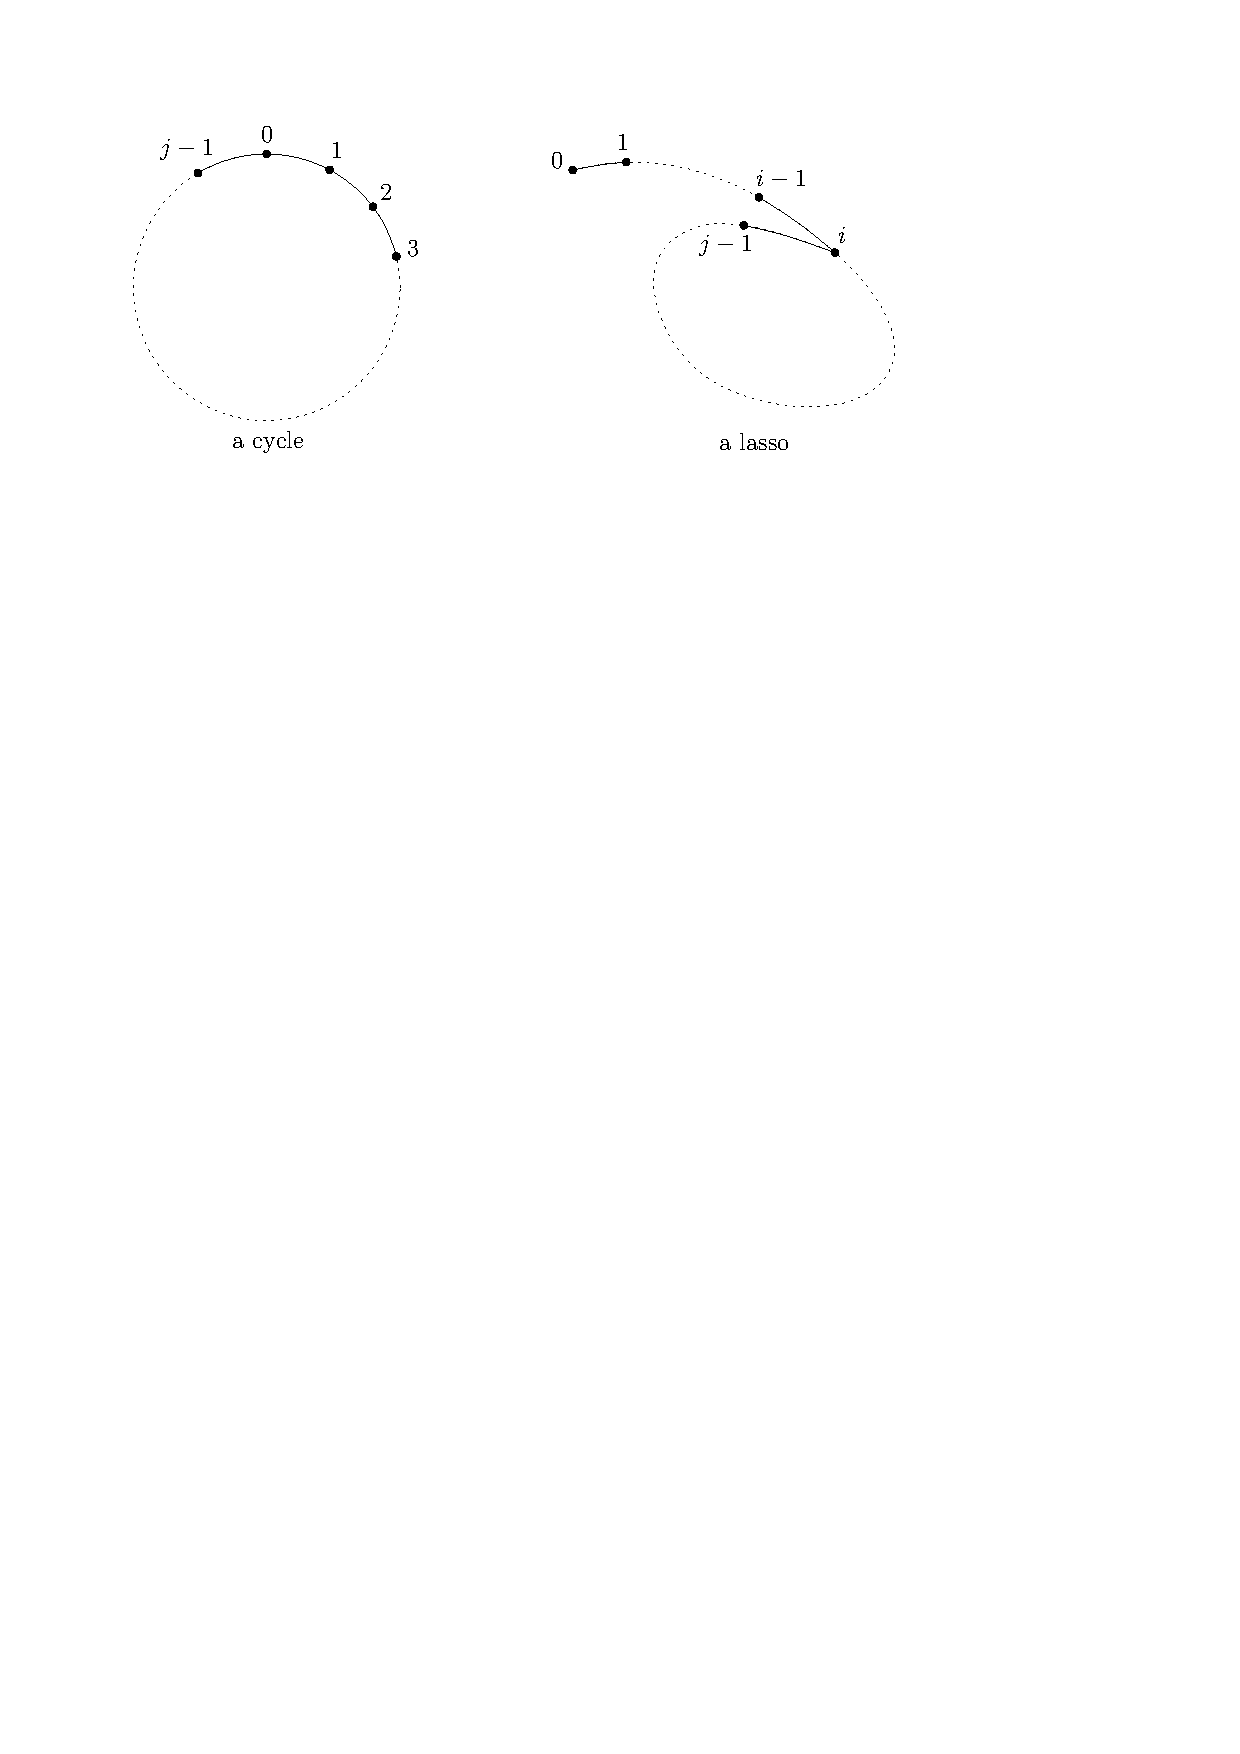
\includegraphics[width=0.8\textwidth]{figures/cycle-and-lasso.pdf}
  \end{center}
  
  Show that a lasso cannot happen. That is, show 
  that the smallest $i$ for which this happens is $0$, i.e, for some $j$ we have
  $F'_0 = F'_j$ and $F'_1 = F'_{j+1}$ and thus $F'_n = F'_{n \textnormal{ mod }  j}$.
\end{exercise}
 \paragraph{Solution}
  If we already know that lasso cannot happen, we can just check $F'_i$ from $1$ to
  $k^2$ until $F'_i = 0$ and $F'_{i+1} = 1$.

  If we do not know that, we can use Floyd Cycle Detection Algorithm. Initialy, 
  we set two pointer $t = (F'_0, F'_1), s = (F'_0, F'_1)$. Every step $t$ become from 
  $(F'_i, F'_{i+1})$  to $(F'_{i+1}, F'_{i+2})$, $s$ become from 
  $(F'_i, F'_{i+1})$  to $(F'_{i+2}, F'_{i+3})$, after every step, check the if t equals s,
  if equals then stop, we already find the cycle.

  $$
    {\displaystyle \mathbf {F} ={\begin{bmatrix}1&1\\1&0\end{bmatrix}}}
  $$
  To prove the lasso cannot happen. we just need to prove the 
  $\exists p > 0, \mathbf{F}^p = I$. 

  $$
    \begin{bmatrix}1&1\\1&0\end{bmatrix}
    \begin{bmatrix}0&1\\1&-1\end{bmatrix}=I
  $$
  So $F$ is invertable, so $F$ is in $GL_2(Z_k)$. Because $GL_2(Z_k)$ is finite, so must
  $\exists a, b(a > b), F^a = F^b$, then $F^{a-b}=I$, so lasso will not happen.
  
\paragraph{Python.} Please write your code in python. It is a very simple programming
language. If you do not know any python, I can put same example code online and 
you can learn by example. Also, for this homework you definitely need a Big Integer class
since numbers with ten thousand digits do not fit into any \texttt{long long int} or similar.
Python automatically supports Big Integer, so there is no problem here.
\begin{verbatim}
  def find_fib_cycle(k):
    """ The lasso cannot happen """
    j = 0
    f0, f1 = 0, 1
    
    while True:
        f0, f1 = f1, (f0 + f1) % k
        if f0 == 0 and f1 == 1:
            return 0, j
        j += 1

  def find_fib_lasso(k):
    """ Floyd Cycle Detection Algorithm """
    i = 0
    j = 0
    t = (0, 1)
    s = (0, 1)
    while True:
        t = (t[1], (t[0] + t[1]) % k)
        s = (s[1], (s[0] + s[1]) % k)
        s = (s[1], (s[0] + s[1]) % k)

        i += 1
        j += 2
        if t == s:
            return i, j
\end{verbatim}

\end{document}
